\documentclass[11pt]{article}
\usepackage[margin=1in]{geometry}
\usepackage{../../styles/isaiah}
\usepackage{../../styles/components/configurableGrid}

\begin{document}

% Isaiah Context Grid
\configurableGrid{2}{Isaiah 1-12}{
    \textbf{\large Chapters 1-5}

    \textit{Judgment and Rebellion}
}{
    \textbf{\large Chapters 6-8}

    \textit{Isaiah's Call \& \\Commission}
}{
    \textbf{\large Chapters 9-12}

    \textit{Hope and Restoration}
}

\newpage
% Overview of Isaiah 6
\begin{overview}{Isaiah 6 — Overview}

\overviewsection[0]{%
\textbf{Verses 1-5: Vision of the Holy King}
\begin{itemize}
    \item Isaiah sees the LORD on His throne with seraphim crying "Holy, holy, holy"
\end{itemize}
}

\overviewsection[1]{%
\textbf{Verses 6-8: Cleansing and Commission}
\begin{itemize}
    \item A seraph cleanses Isaiah's lips with a coal from the altar
    \item Isaiah responds to God's call: "Here I am! Send me."
\end{itemize}
}

\overviewsection[0]{%
\textbf{Verses 9-13: The Hard Message}
\begin{itemize}
    \item God gives Isaiah a difficult message of judgment
    \item The people will hear but not understand until the land is desolate
\end{itemize}
}

\end{overview}
\newpage
% Verses 1-5 - Chiastic Structure
\begin{chiasticoutline}[Isaiah 6:1-5]{.75em}{2em}

    \chiasticverselabel[A]{0}{
\versenum{1} In the year that \highlightblue{King} Uzziah died I saw the Lord \highlightgreen{sitting} upon a throne, high and lifted up; and the train of his robe filled the temple.
    }{Seen the King}

    \chiasticverselabel[B]{1}{
\versenum{2} Above him stood the seraphim. Each had six wings: with two he covered his face, and with two he covered his feet, and with two he flew.
\versenum{3} And one called to another and said: ``Holy, holy, holy is the LORD of hosts; the whole earth is full of his glory!''
\versenum{4} And the foundations of the thresholds shook at the voice of him who called, and the house was filled with smoke.
    }{Holy, Holy, Holy}

    \chiasticverselabel[A']{0}{
\versenum{5} And I said: ``Woe is me! For I am lost; for I am a man of unclean lips, and I \highlightgreen{dwell} in the midst of a people of unclean lips; for my eyes have seen the \highlightblue{King}, the LORD of hosts!''
    }{Seen the King}

\end{chiasticoutline}

{\vspace{1em}}

{\large\bfseries The Real King}
{\vspace{1em}}

King Uzziah had reigned for 52 years when he died, making him one of the longest-reigning kings of Judah. His death marked the end of an era of prosperity and stability. But in this moment of political uncertainty, Isaiah sees the true King - the LORD of hosts - seated on His eternal throne.

{\vspace{1em}}
Right before King Uzziah died though, we read the following story in 2 Chronicles 26:16-21:

{\vspace{1em}}

\subsectionheader{2 Chronicles 26:16-21}

\begin{versesection}{2em}

\versenum{16} "But when he was strong, he grew proud, to his destruction. For he was unfaithful to the LORD his God and entered the temple of the LORD to burn incense on the altar of incense. \versenum{17} But Azariah the priest went in after him, with eighty priests of the LORD who were men of valor. \versenum{18} And they withstood King Uzziah and said to him, "It is not for you, Uzziah, to burn incense to the LORD, but for the priests, the sons of Aaron, who are consecrated to burn incense. Go out of the sanctuary, for you have done wrong, and it will bring you no honor from the LORD God." \versenum{19} Then Uzziah was angry, and he had a censer in his hand to burn incense. And when he became angry with the priests, leprosy broke out on his forehead in the presence of the priests in the house of the LORD, by the altar of incense. \versenum{20} And Azariah the chief priest and all the priests looked at him, and behold, he was leprous in his forehead. And they rushed him out quickly, and he himself hurried to go out because the LORD had struck him. \versenum{21} And King Uzziah was a leper to the day of his death, and being a leper lived in a separate house, for he was excluded from the house of the LORD. And Jotham his son was over the king's household, governing the people of the land.

\end{versesection}

{\vspace{1em}}

One of the reasons Isaiah could be explicitly calling out that this occurred the day of King Uzziah's death could be contrasting what Isaiah himself is going through here in God's holy place vs how King Uzziah treated it.

{\vspace{1em}}
It's also maybe "ironic" in a way that as a leper, you'd have "Unclean" come out of your lips in order to let others know to stay away. Here Isaiah says he has the same – the remedy isn't to "burn incense" for yourself, it's to have God's atoning mercy given to you.

{\vspace{3em}}
{\large\bfseries Isaiah's Response to Holiness}
{\vspace{1em}}

Why does Isaiah say he's "lost" in response to what he's just witnessed? It's helpful to compare translations when doing a deeper study.
If you see a big difference in wording in the translations, odds are the underlying Hebrew word has a bit more nuance than can easily be communicated with just a single word or two in English.
\begin{biblecomparison}{Isaiah 6:5a}
\translation{ESV}{And I said: "Woe is me! For I am lost;"}
\translation{NASB}{"Then I said, "Woe to me, for I am ruined!"}
\translation{NIV}{"Woe to me!" I cried. "I am ruined!"}
\translation{KJV}{Then said I, Woe is me! for I am undone;}
\translation{NET}{I said, "Woe to me! I am destroyed,"}
\end{biblecomparison}

\hebrewword{Lost}{דָּמָה}{da.mah}{Ceased, cut off, or destroyed. Crushed into nonexistence}

What does the holiness of God even mean? It's his "otherness" – He's set apart in that He's filled with such extreme goodness and purity. Kind of like the sun that can be incredibly powerful and dangerous, but is also the source of life.

This is why Isaiah is so terrified – how can he be able to live in the presence of a Holy God?
\newpage
{\large\bfseries Isaiah and the "People"}
{\vspace{1em}}

After he spent just about all of chapters 1-5 roasting Israel and clearly painting their need for judgement, when confronted with the holiness of Yahweh directly, he doesn't just say "Woe is Israel", he identifies his individualistic role within the larger community.
\newpage

% Verses 6-8 - Biblical Outline
\begin{biblicaloutline}[Isaiah 6:6-8]
    
        \versenum{6} Then one of the seraphim flew to me, having in his hand a burning coal that he had taken with tongs from the altar.
        \versenum{7} And he touched my mouth and said: ``Behold, this has touched your lips; your guilt is taken away, and your sin atoned for.''
         \versenum{8} And I heard the voice of the Lord saying, ``Whom shall I send, and who will go for us?'' Then I said, ``Here I am! Send me.''

\end{biblicaloutline}


{\vspace{2em}}
{\large\bfseries Holiness Transfer}

{\vspace{1em}}

\begin{quote}
\textit{"Instead of the temple becoming contaminated
by Isaiah’s impurity, the opposite happens: God’s
holiness transfers to Isaiah and erases his sin and
impurity.\\\\This is unexpected to say the least! The implications of Isaiah's vision are huge.
  Perhaps God doesn't need to be protected by the impurity our
  sin, maybe it's the other way around. Maybe it's our sin that
   is endangered by God's holiness."}\\\\
\hfill --- Bible Project, \textit{Holiness Study Guide}, https://bibleproject.com/videos/holiness/
\end{quote}


{\vspace{2em}}
{\large\bfseries Guarding the Thresholds}


{\vspace{1em}}

\subsectionheader{Genesis 3:22-24}

\begin{versesection}{2em}

\versenum{22} "Then the LORD God said, "Behold, the man has become like one of us in knowing good and evil. Now, lest he reach out his hand and take also of the tree of life and eat, and live forever—" \versenum{23} therefore the LORD God sent him out from the garden of Eden to work the ground from which he was taken. \versenum{24} He drove out the man, and at the east of the garden of Eden he placed the cherubim and a flaming sword that turned every way to guard the way to the tree of life."

\end{versesection}


\begin{center}
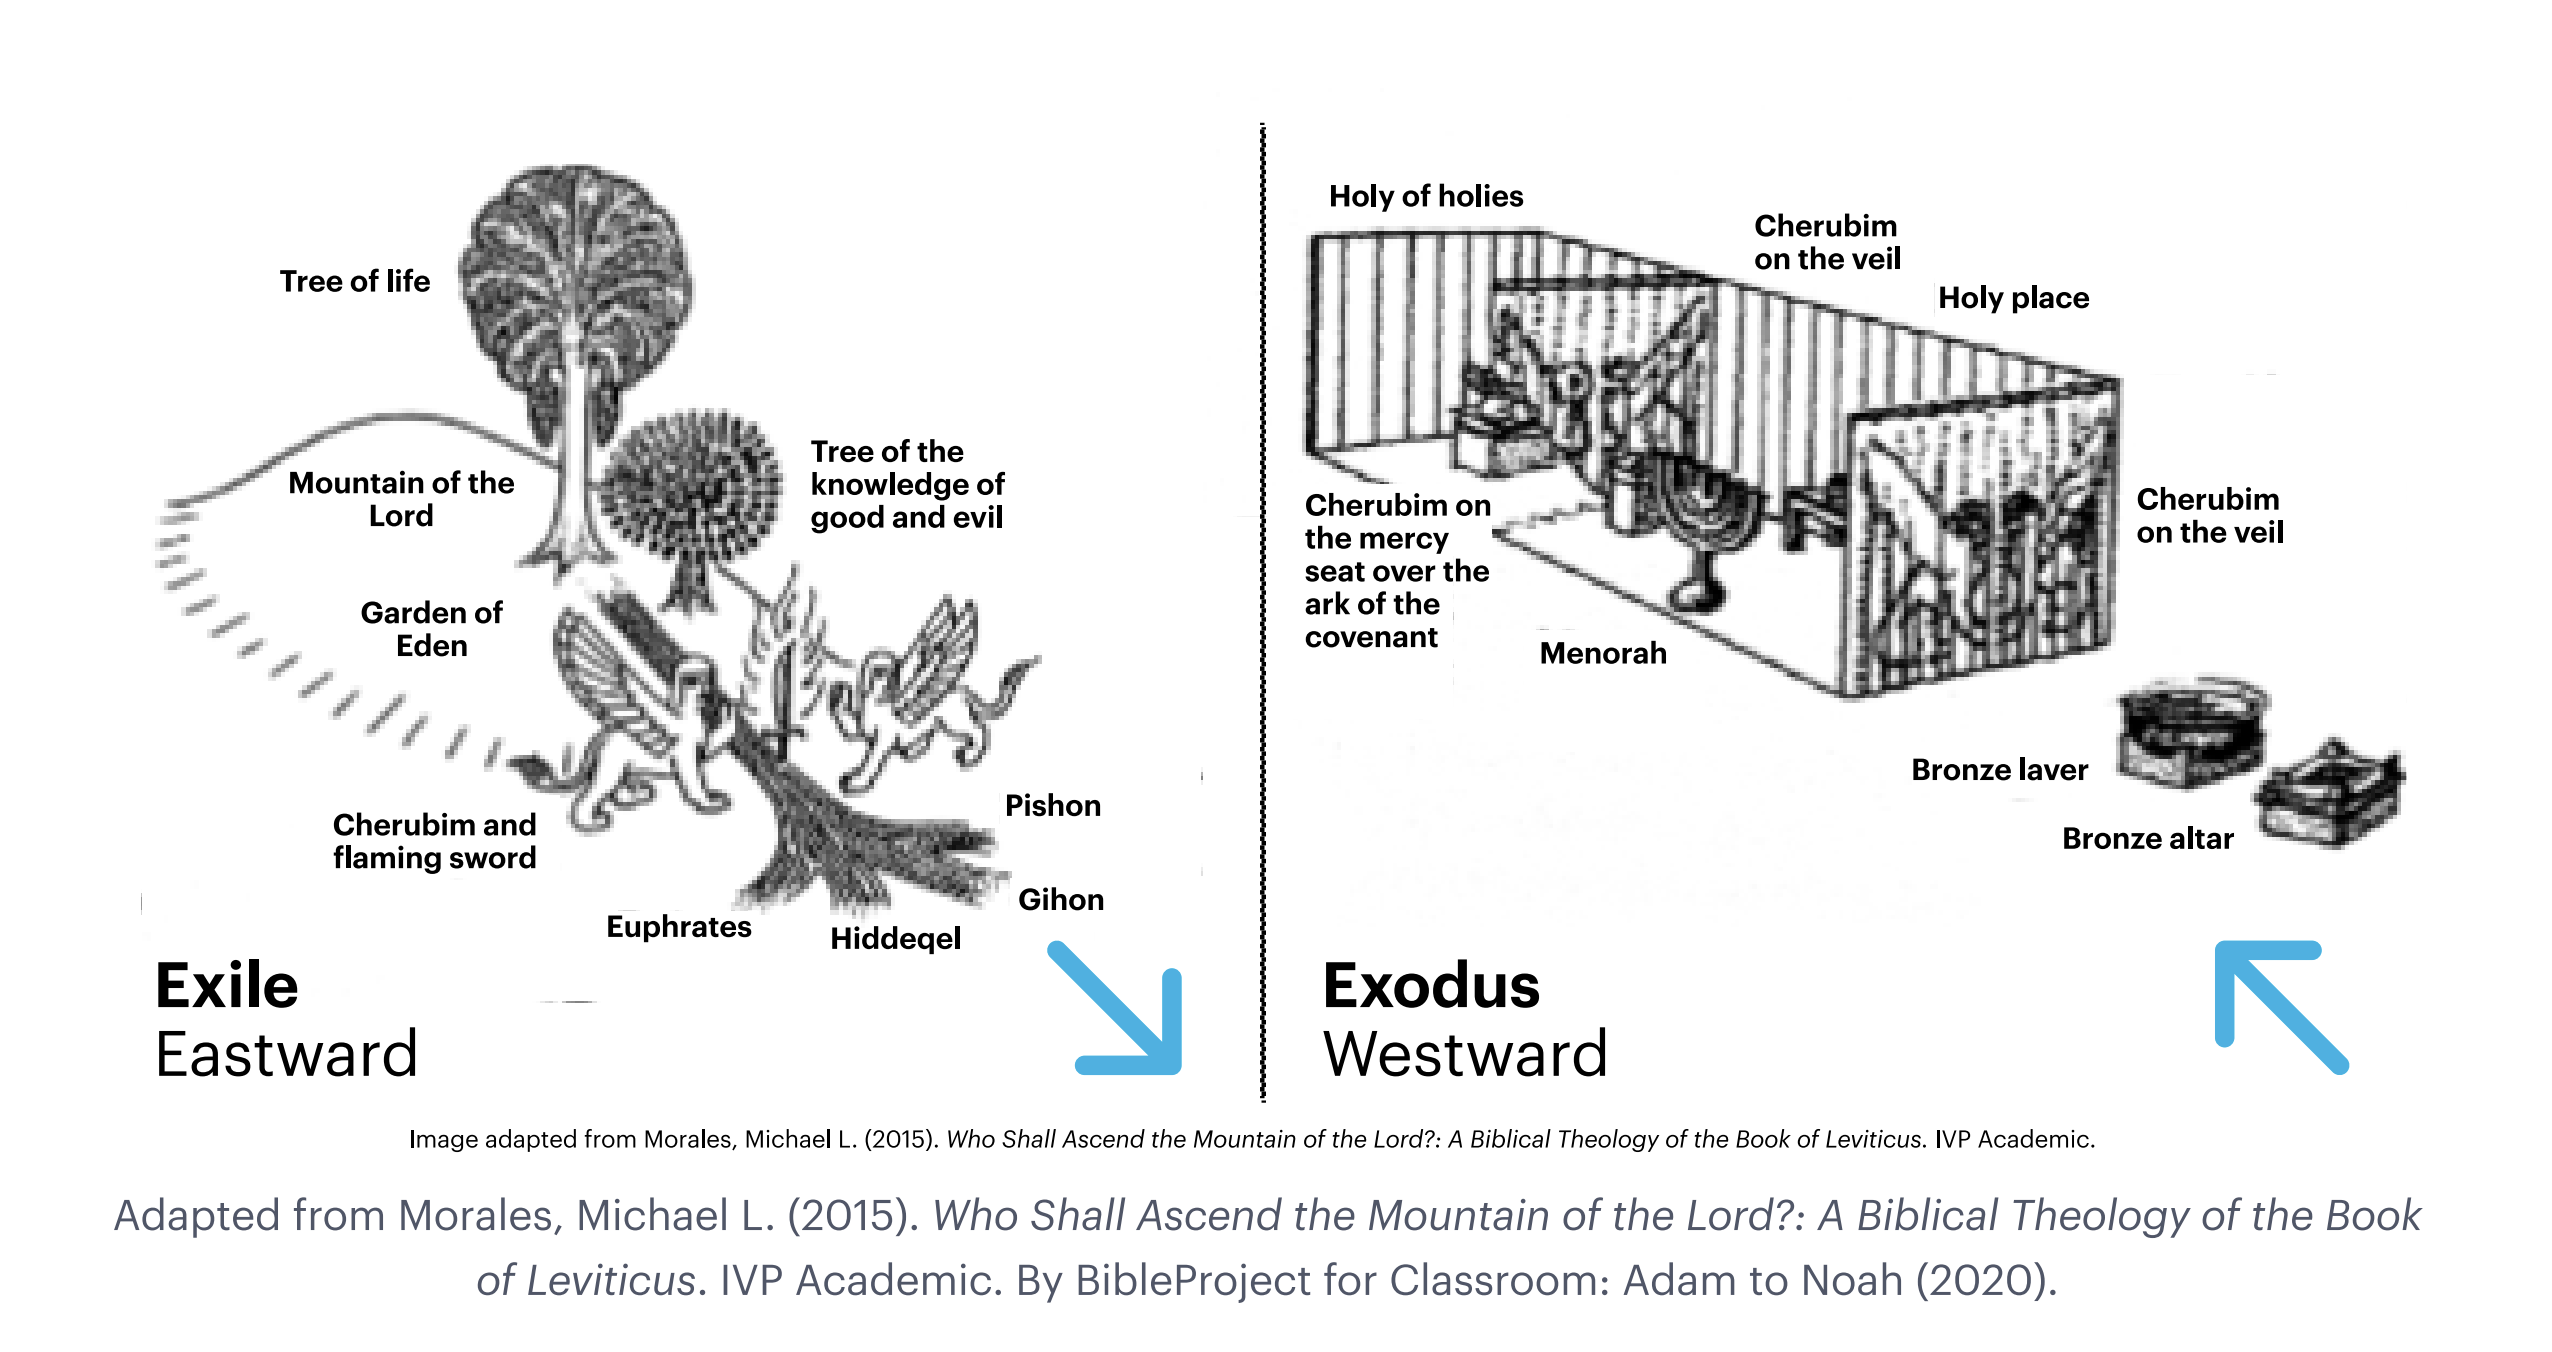
\includegraphics[width=0.8\textwidth]{eden-temple.png}
\end{center}

{\vspace{2em}}

This isn't the first time we read about angelic beings who guard the sacred space of God. Here we have the guardians of the tree of life set up where Adam and Eve forfeited their right to have perfect communion with God Himself.

Now, Isaiah is "back in the garden" so to speak, by being directly before Yahweh. But he still needs to "pass through the cherubim" in order to be cleansed and begin his ministry.

These are guardians of the "entryway" or "threshold" which is probably why the foundations of the thresholds are specifically called out in v4.


\newpage
% Verses 9-13 - Biblical Outline
\begin{biblicaloutline}[Isaiah 6:9-13]
    
    \subsectionheader{The Hard Message (9-10)}

    \begin{versesection}{2em}
        \versenum{9} And he said, ``Go, and say to this people: `Keep on hearing, but do not understand; keep on seeing, but do not perceive.'

        \versenum{10} Make the heart of this people dull, and their ears heavy, and blind their eyes; lest they see with their eyes, and hear with their ears, and understand with their hearts, and turn and be healed.''
    \end{versesection}
    
    \subsectionheader{How Long? (11-13)}
    
    \begin{versesection}{2em}
        \versenum{11} Then I said, ``How long, O Lord?'' And he said: ``Until cities lie waste without inhabitant, and houses without people, and the land is a desolate waste,

        \versenum{12} and the LORD removes people far away, and the forsaken places are many in the midst of the land.

        \versenum{13} And though a tenth remain in it, it will be burned again, like a terebinth or an oak, whose stump remains when it is felled.'' The holy seed is its stump.
    \end{versesection}

\end{biblicaloutline}
\newpage

{\large\bfseries Keep on Hearing}

{\vspace{1em}}

Verses 9-10 are picked up by Jesus in a few places in the Gospels:

{\vspace{1em}}
\subsectionheader{Matthew 13:10-17}

\begin{versesection}{2em}

\versenum{10} "Then the disciples came and said to him, `Why do you speak to them in parables?' \versenum{11} And he answered them, `To you it has been given to know the secrets of the kingdom of heaven, but to them it has not been given. \versenum{12} For to the one who has, more will be given, and he will have an abundance, but from the one who has not, even what he has will be taken away. \versenum{13} This is why I speak to them in parables, because seeing they do not see, and hearing they do not hear, nor do they understand. \versenum{14} Indeed, in their case the prophecy of Isaiah is fulfilled that says: \\\\`You will indeed hear but never understand,\\ \poetryline{} and you will indeed see but never perceive.'\\ \versenum{15} For this people's heart has grown dull,\\ \poetryline{} and with their ears they can barely hear,\\ \poetryline{} and their eyes they have closed, \\ lest they should see with their eyes \\ \poetryline{} and hear with their ears\\ and understand with their heart\\ \poetryline{} and turn, and I would heal them.'"
\end{versesection}

{\vspace{1em}}
And in John, the same thing is present, except this time, John brings extra commentary to the surrounding passage in Isaiah 6:

\begin{versesection}{2em}

\subsectionheader{John 12:36-43}

\versenum{36} "While you have the light, believe in the light, that you may become sons of light.” When Jesus had said these things, he departed and hid himself from them. \versenum{37} Though he had done so many signs before them, they still did not believe in him, \versenum{38} so that the word spoken by the prophet Isaiah might be fulfilled:\\\\ “Lord, who has believed what he heard from us,\\ \poetryline{} and to whom has the arm of the Lord been revealed?” \\\\ \versenum{39} Therefore they could not believe. For again Isaiah said,\\\\ \versenum{40} “He has blinded their eyes\\ \poetryline{} and hardened their heart,\\ lest they see with their eyes\\ \poetryline{} and understand with their heart, and turn,\\ \poetryline{} and I would heal them.”\\\\ \versenum{41} Isaiah said these things because he saw his glory and spoke of him. \versenum{42} Nevertheless, many even of the authorities believed in him, but for fear of the Pharisees they did not confess it, so that they would not be put out of the synagogue; \versenum{43} for they loved the glory that comes from man more than the glory that comes from God.

\end{versesection}

{\vspace{2em}}
{\large\bfseries The Holy Seed}

{\vspace{1em}}

In spite of this rejection and hardening, this glorious passage ends with a glorious promise, a holy seed (offspring) will remain from the chopped-down tree. Just like how the vision of Yahweh is 3x Holy, so the remnant after destruction will be.

Out of death and judgement comes the promise of a new life. A life that is holy and dedicated to the Lord!

\begin{quote}
\textit{"We come nearer to the heart of
this chapter by noting that it is pervaded by the thought of death:
the dying king (1), the prophet under sentence of death (5), the sacrificial animal dead on the altar (6) and the felled tree (I3). Twice over,
death seems to spell the end but is found not to be so. The king lies
dead (1) but it turns out to be only the felling of a tree, and life
remains in the root (13); the prophet lies dead, struck down by sin
under divine holiness (5) but when the seraph approaches, apparently
bearing the fire of judgment, it is to apply the efficacy of a sacrifice
for sin and to speak the word 'atoned' (7). Death does not have the
last word."}\\\\
\hfill  --- Barry Webb, \textit{The Message of Isaiah}
\end{quote}

\begin{thesauce}
\sauceitem{Seraph means "to burn" and this is the same word used in the fiery serpent on the pole that healed Israel from their snake bites in Numbers 21. There's maybe some interesting things here with the purifying nature of both of these stories – or even how Jesus uses this story in John 3:14-15.}

\sauceitem{How does Isaiah's call narrative relate to Moses's? Both have the firey holiness of God, both have a servant who responds to God's commissioning of them to give a hard message. What other comparisions are there to meditate on?}

\sauceitem{What does the hardening of the hearers of this message mean for God's Sovereignty vs Human Responsibility? Why couldn't the message be like chapter 1:16 where they could turn and repent and be clean? Is this message to the same people?}

\sauceitem{Isaiah let's out the 7th "Woe" picking up from the 6 previous ones in chapter 5.}

\end{thesauce}

\end{document}